\chapter{Discussion}\label{cha: discussion}
\noindent
\section{Firmware Evaluation}
The threshold scan confirms that the firmware allows for the configuration of the Citiroc1A ASICs.
\newline
Furthermore, several tests were performed to verify successful configuration of the Citiroc1A ASICs by the FPGAs,
such as disabling specific stages of the ASICs and routing probe signals using the probe register, as detailed in Section \ref{sec:probe_register}.
\section{Frontend Electronics Characterization}
\subsection{Comparison with Testboard Measurments} 
A comparison of the threshold scan to one performed with the same configuration of the Citiroc1A ASIC on a by Weeroc provieded testboard with gain 58 is shown in Figure \ref{fig:threshold_scan_comparison_58}.% and 62 is shown in Figures \ref{fig:threshold_scan_comparison_58} and \ref{fig:threshold_scan_comparison_62}. 
\begin{figure}[H]
    \centering
    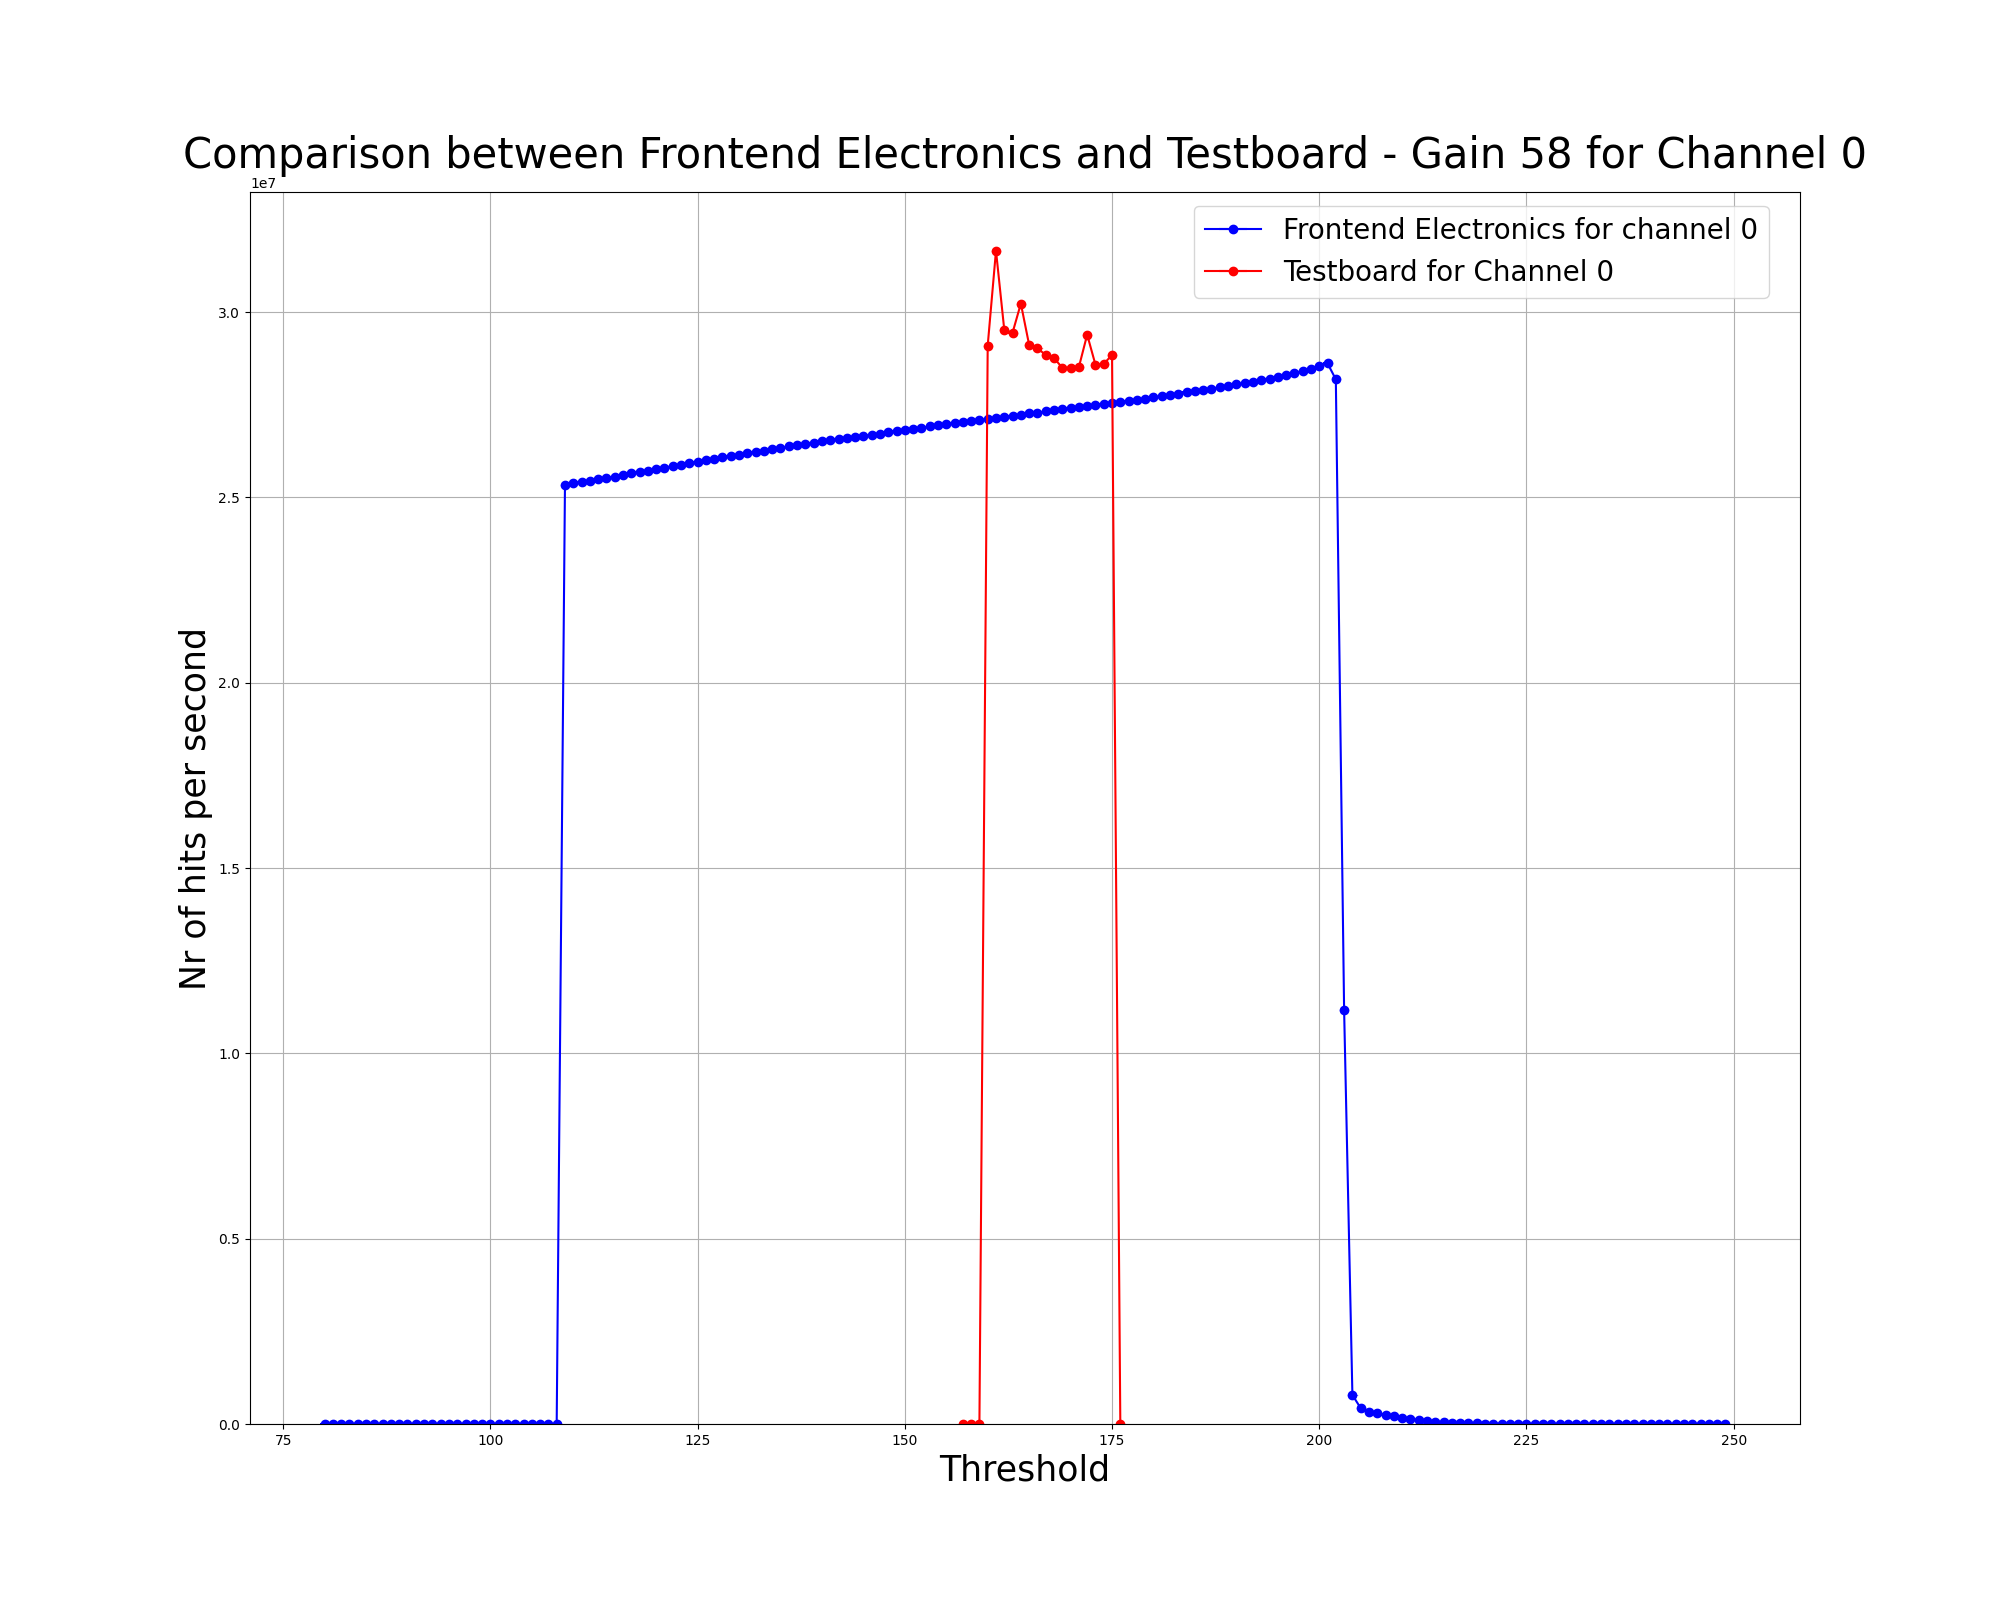
\includegraphics[width=1.0\textwidth]{Runs_170_400_Gain_58.0_0_Channel_compare.png}
    \caption{Comparison of the threshold scan of the frontend electronics to the threshold scan performed on a by Weeroc provided testboard with a gain of 58.}
    \label{fig:threshold_scan_comparison_58}
\end{figure}

%\begin{figure}[H]
 %   \centering
 %   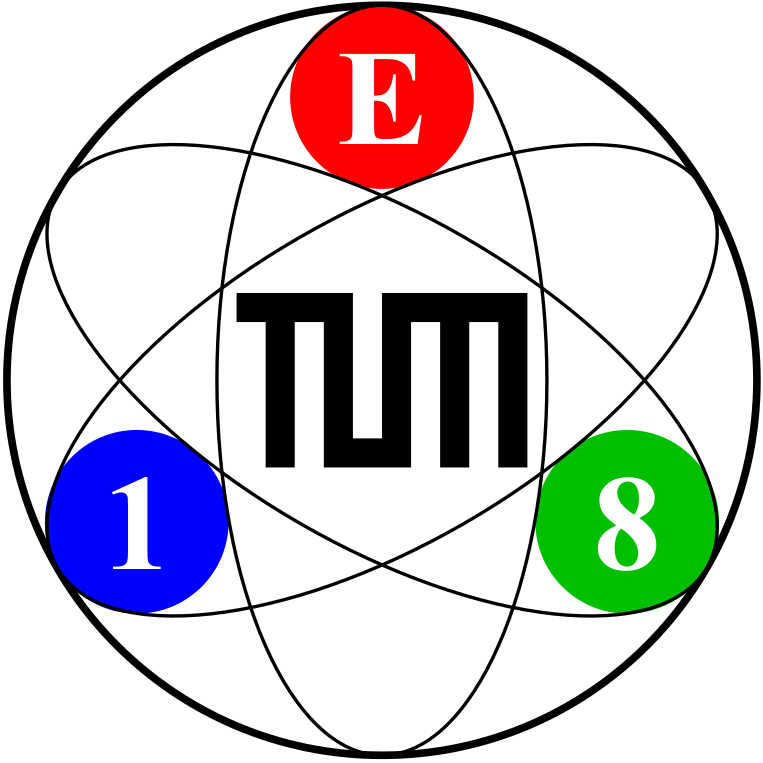
\includegraphics[width=0.8\textwidth]{E18Logo.png}
 %   \caption{Comparison of the threshold scan of the Citiroc1A ASICs of FPGA 1 and 2 to a threshold scan performed on a by Weeroc provided testboard with a gain of 62.}
 %   \label{fig:threshold_scan_comparison_62}
%\end{figure}
The pedestal of the threshold scan performed with the frontend electronics is far larger than the pedestal of the threshold scan performed with the by testboard.
This difference in the observed behavior of the frontend electronics can currently not be explained.
The possibility of the Citiroc1A being wrongly configured was investigated and ruled out by testing for specific behaviors.
Further tests with an oscilloscope probe showed significant high frequency noise on the input signals of the Citiroc1A ASICs,
which could be the cause of the observed behavior, but further investigation is required.(Old noise explenation new explenation needed)

\subsection{S-curve Analysis}
In order to determine the optimal threshold and characterize the noise of the Citiroc1A ASICs of FPGA 1 and 2, an S-curve analysis was performed.
\newline
The falling edge of the pedestal was fitted with the S-curve described in Section \ref{sec:noise_theory}
\newline
The results of the S-curve analysis are shown exemplary for channel 0 of Citiroc1A 1 of FPGA 1 with gain 60,61 and 62 in Figures \ref{fig:S_curve_60}, \ref{fig:S_curve_61} and \ref{fig:S_curve_62}.

\begin{figure}[H]
    \centering
    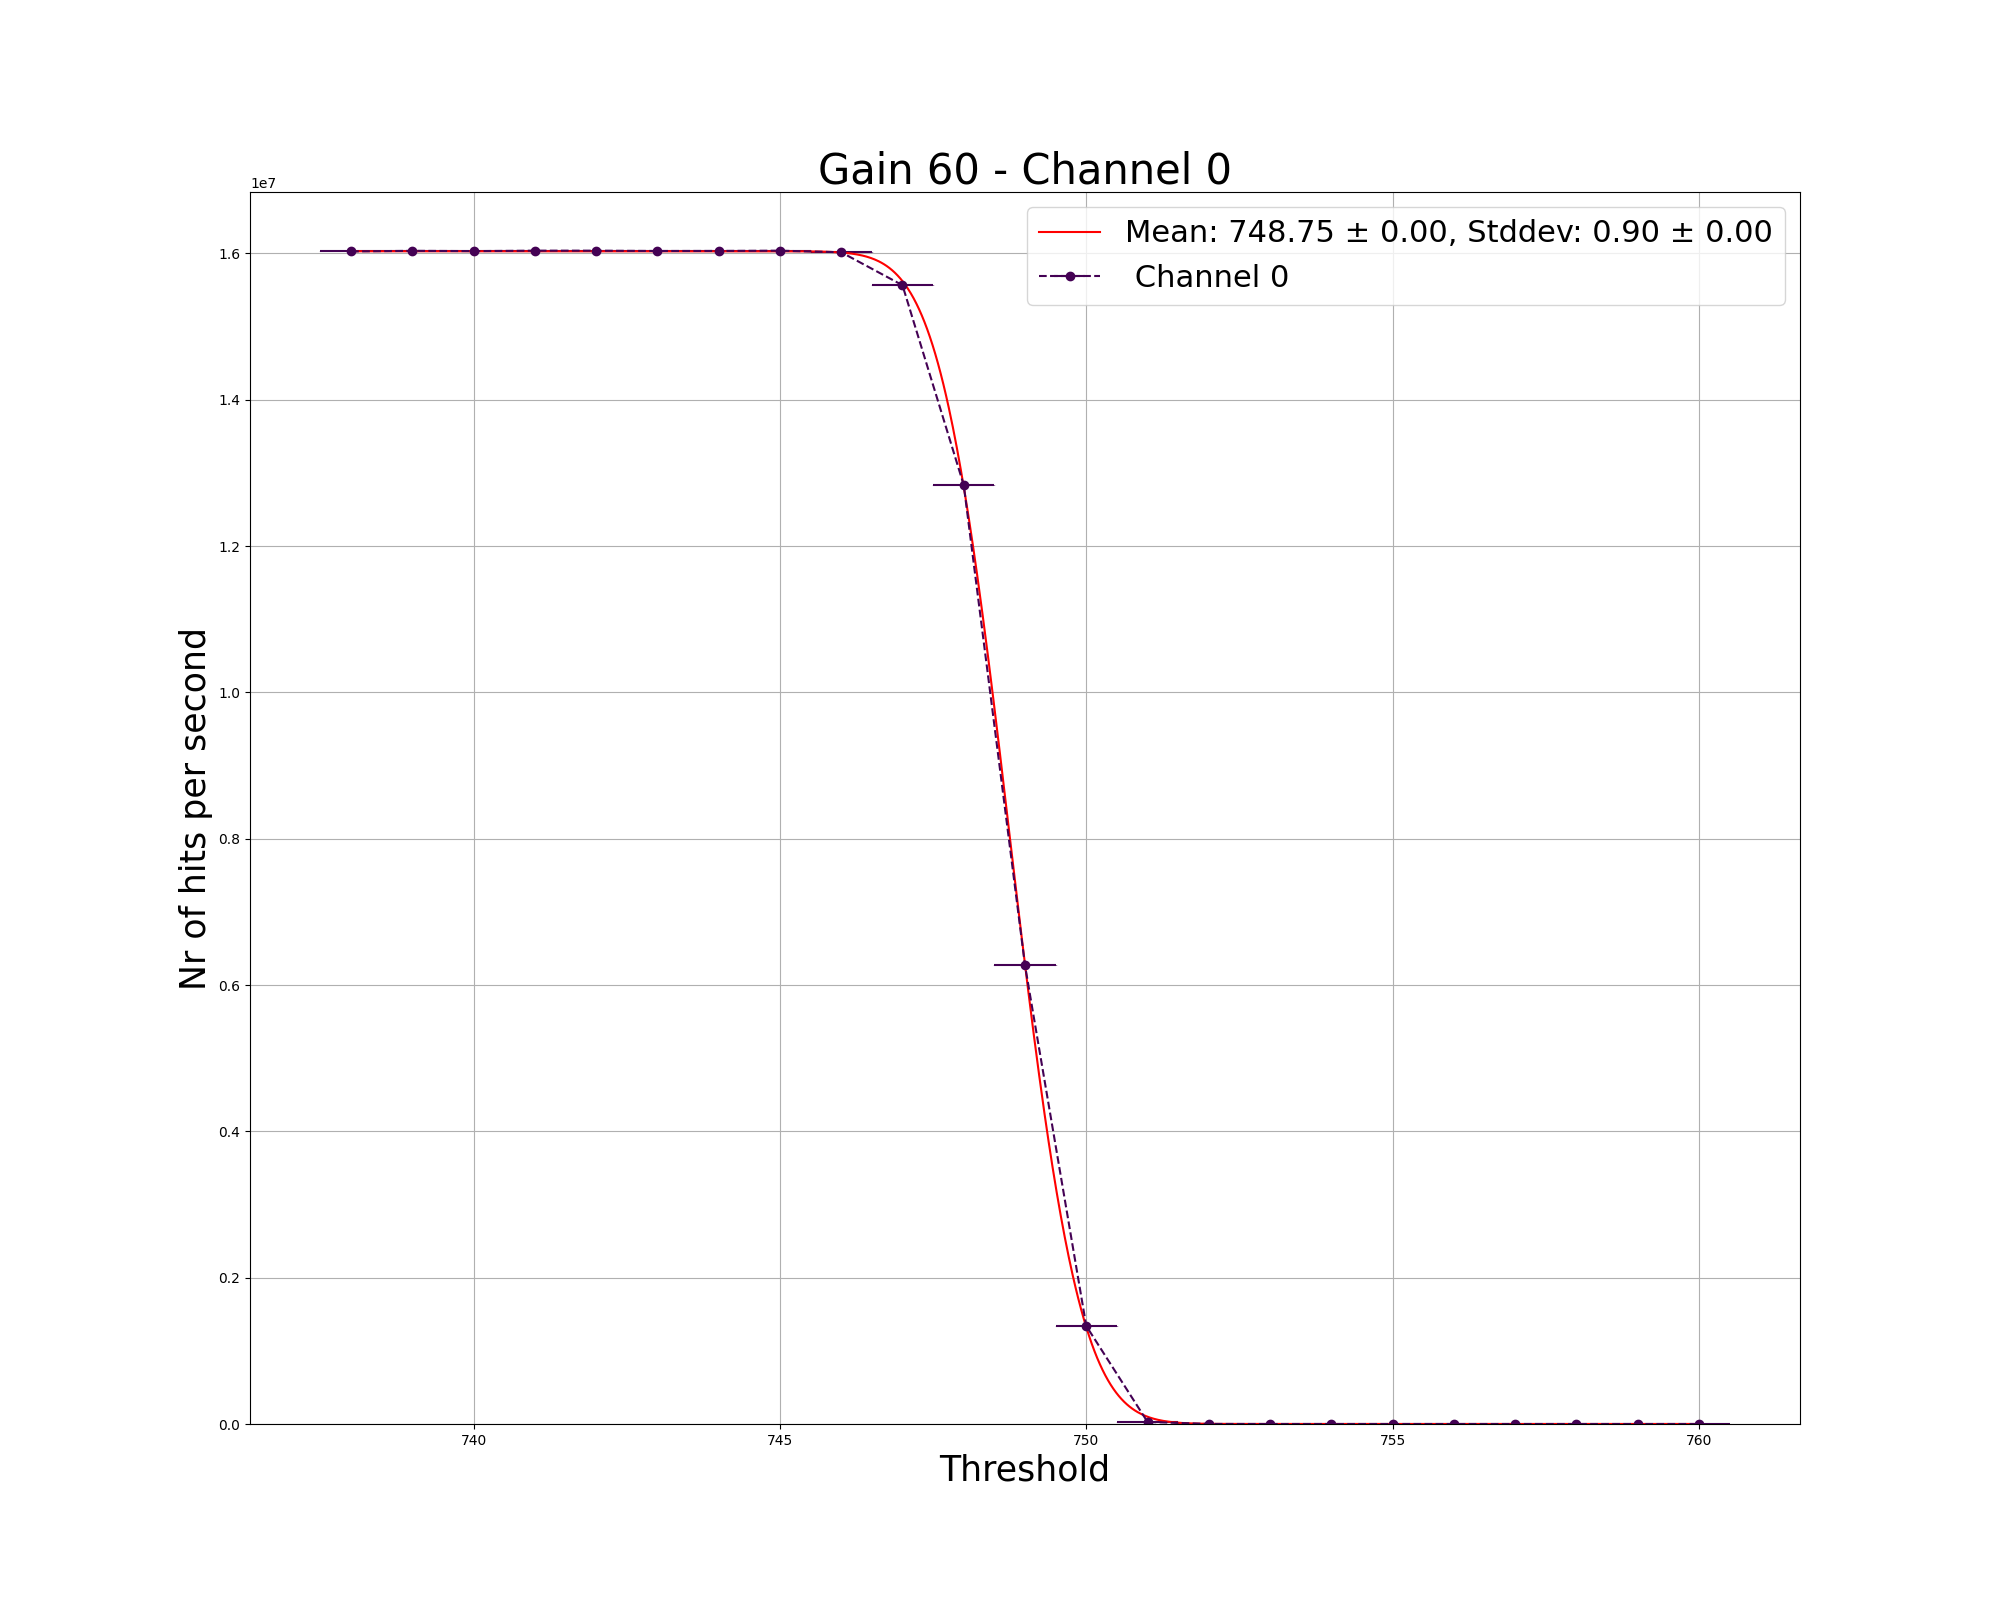
\includegraphics[width=0.7\textwidth]{Runs_170_400_Gain_60.0_0_ChannelALL_FPGAS.png}
    \caption{Results of the S-curve analysis for channel 0 of Citiroc1A 1 of FPGA 1 with gain 60.}
    \label{fig:S_curve_60}
\end{figure}
\begin{figure}[H]
    \centering
    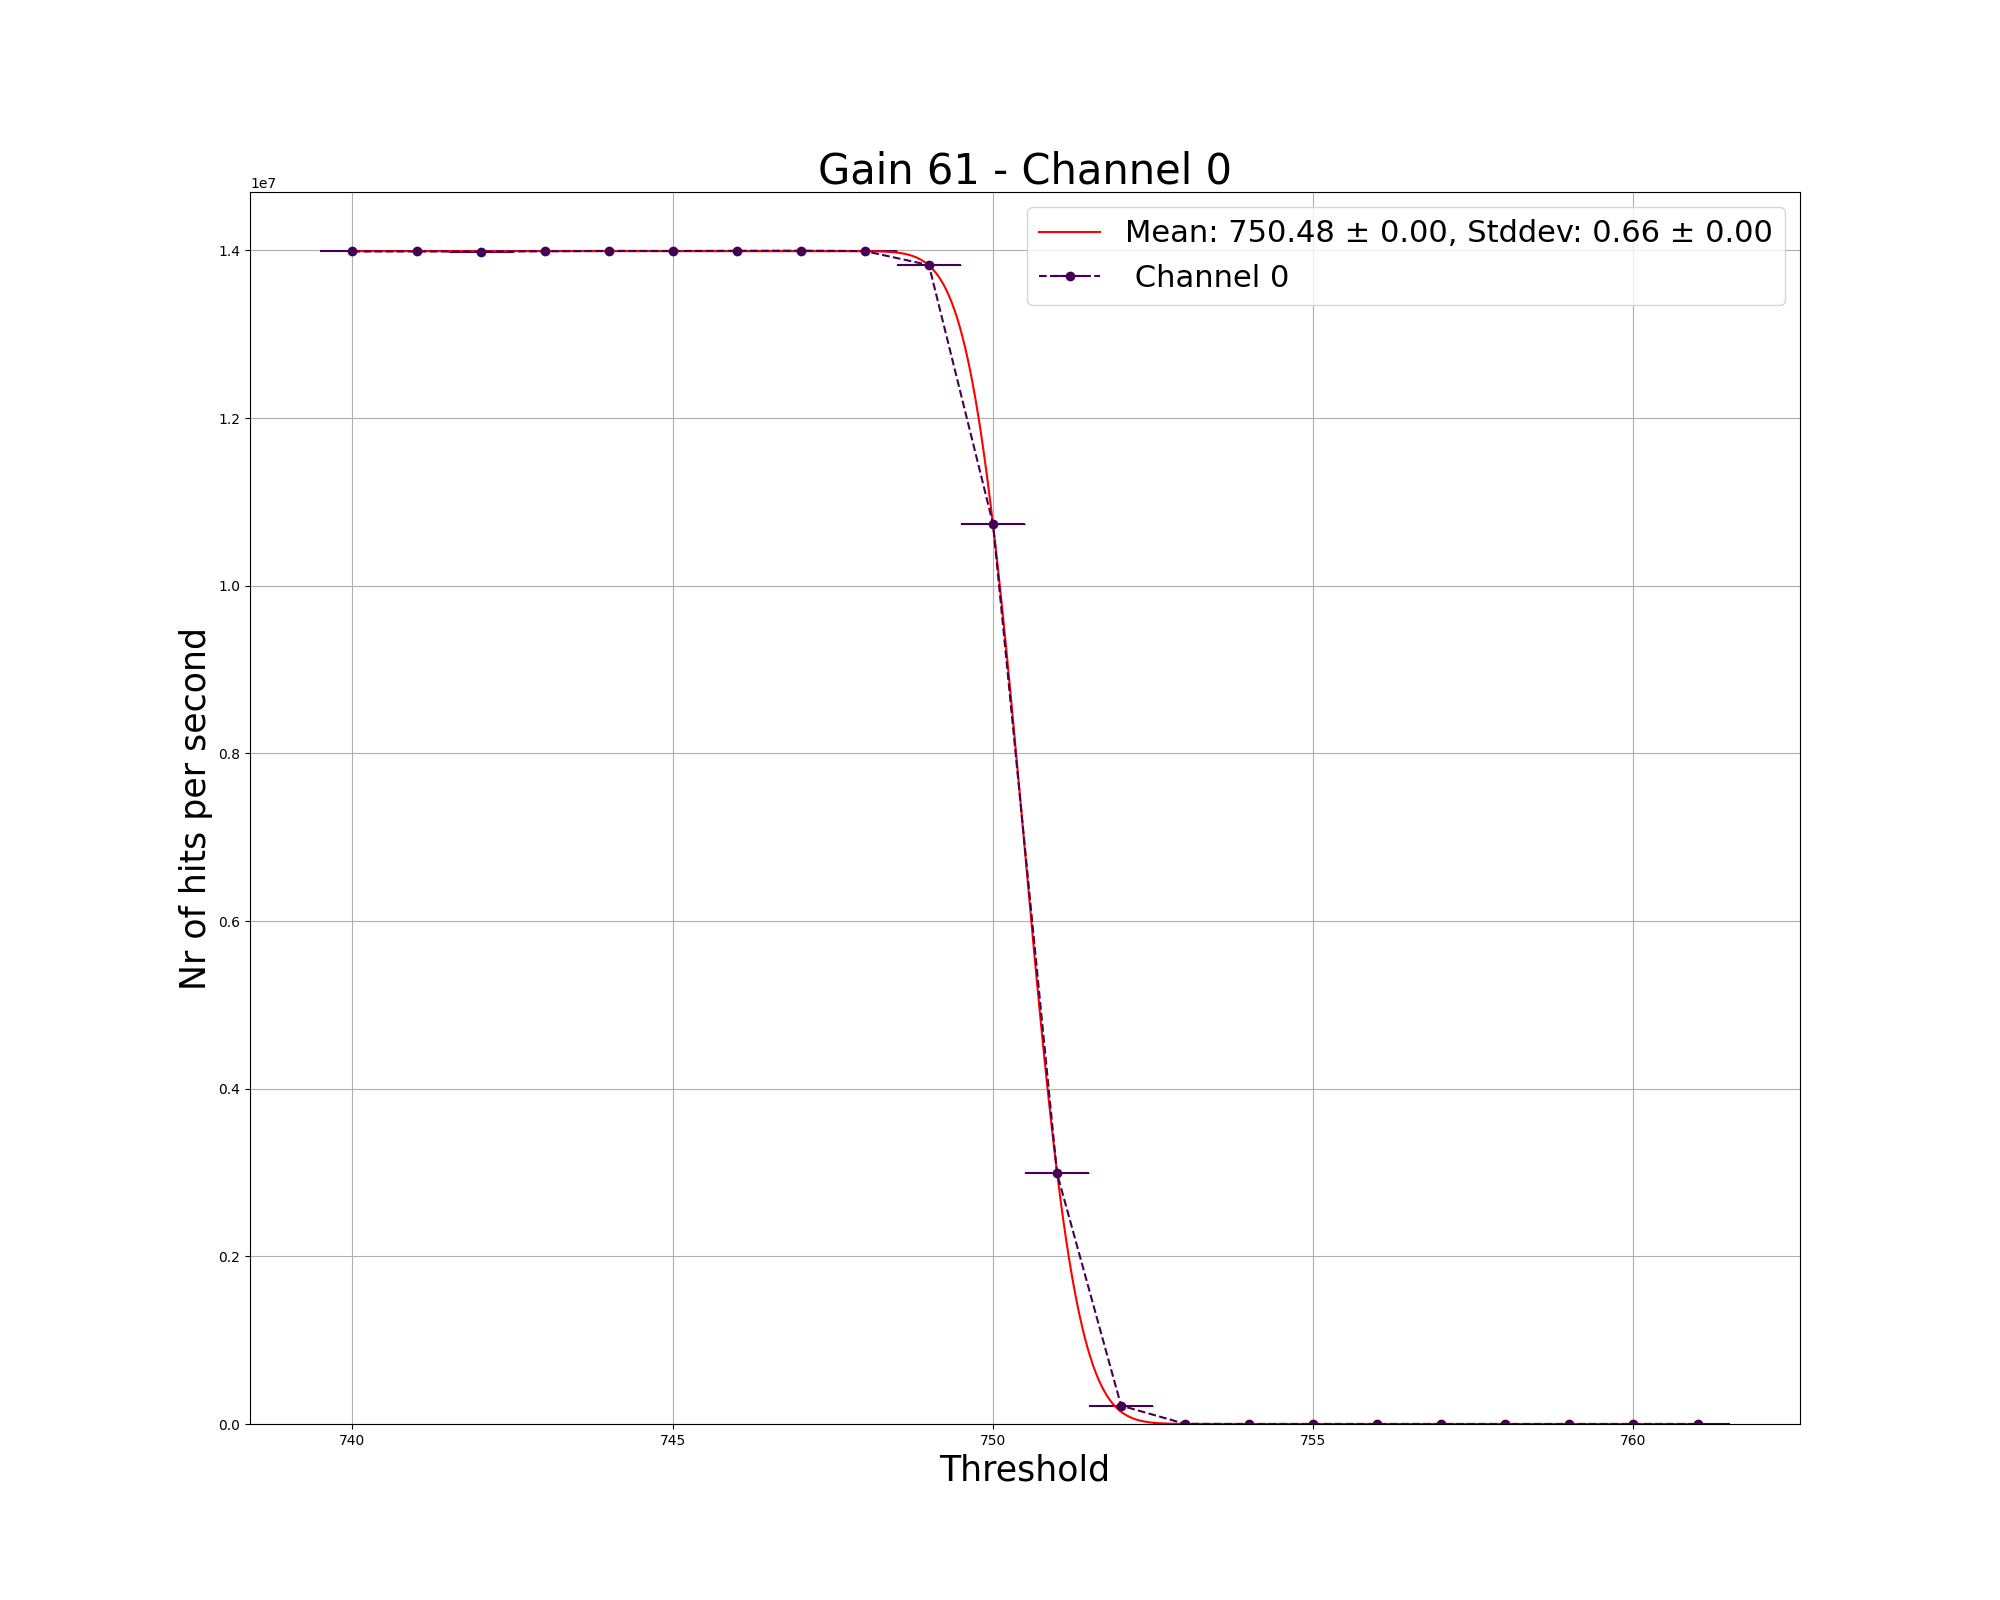
\includegraphics[width=0.7\textwidth]{Runs_170_400_Gain_61.0_0_ChannelALL_FPGAS.png}
    \caption{Results of the S-curve analysis for channel 0 of Citiroc1A 1 of FPGA 1 with gain 61.}
    \label{fig:S_curve_61}
\end{figure}
\begin{figure}[H]
    \centering
    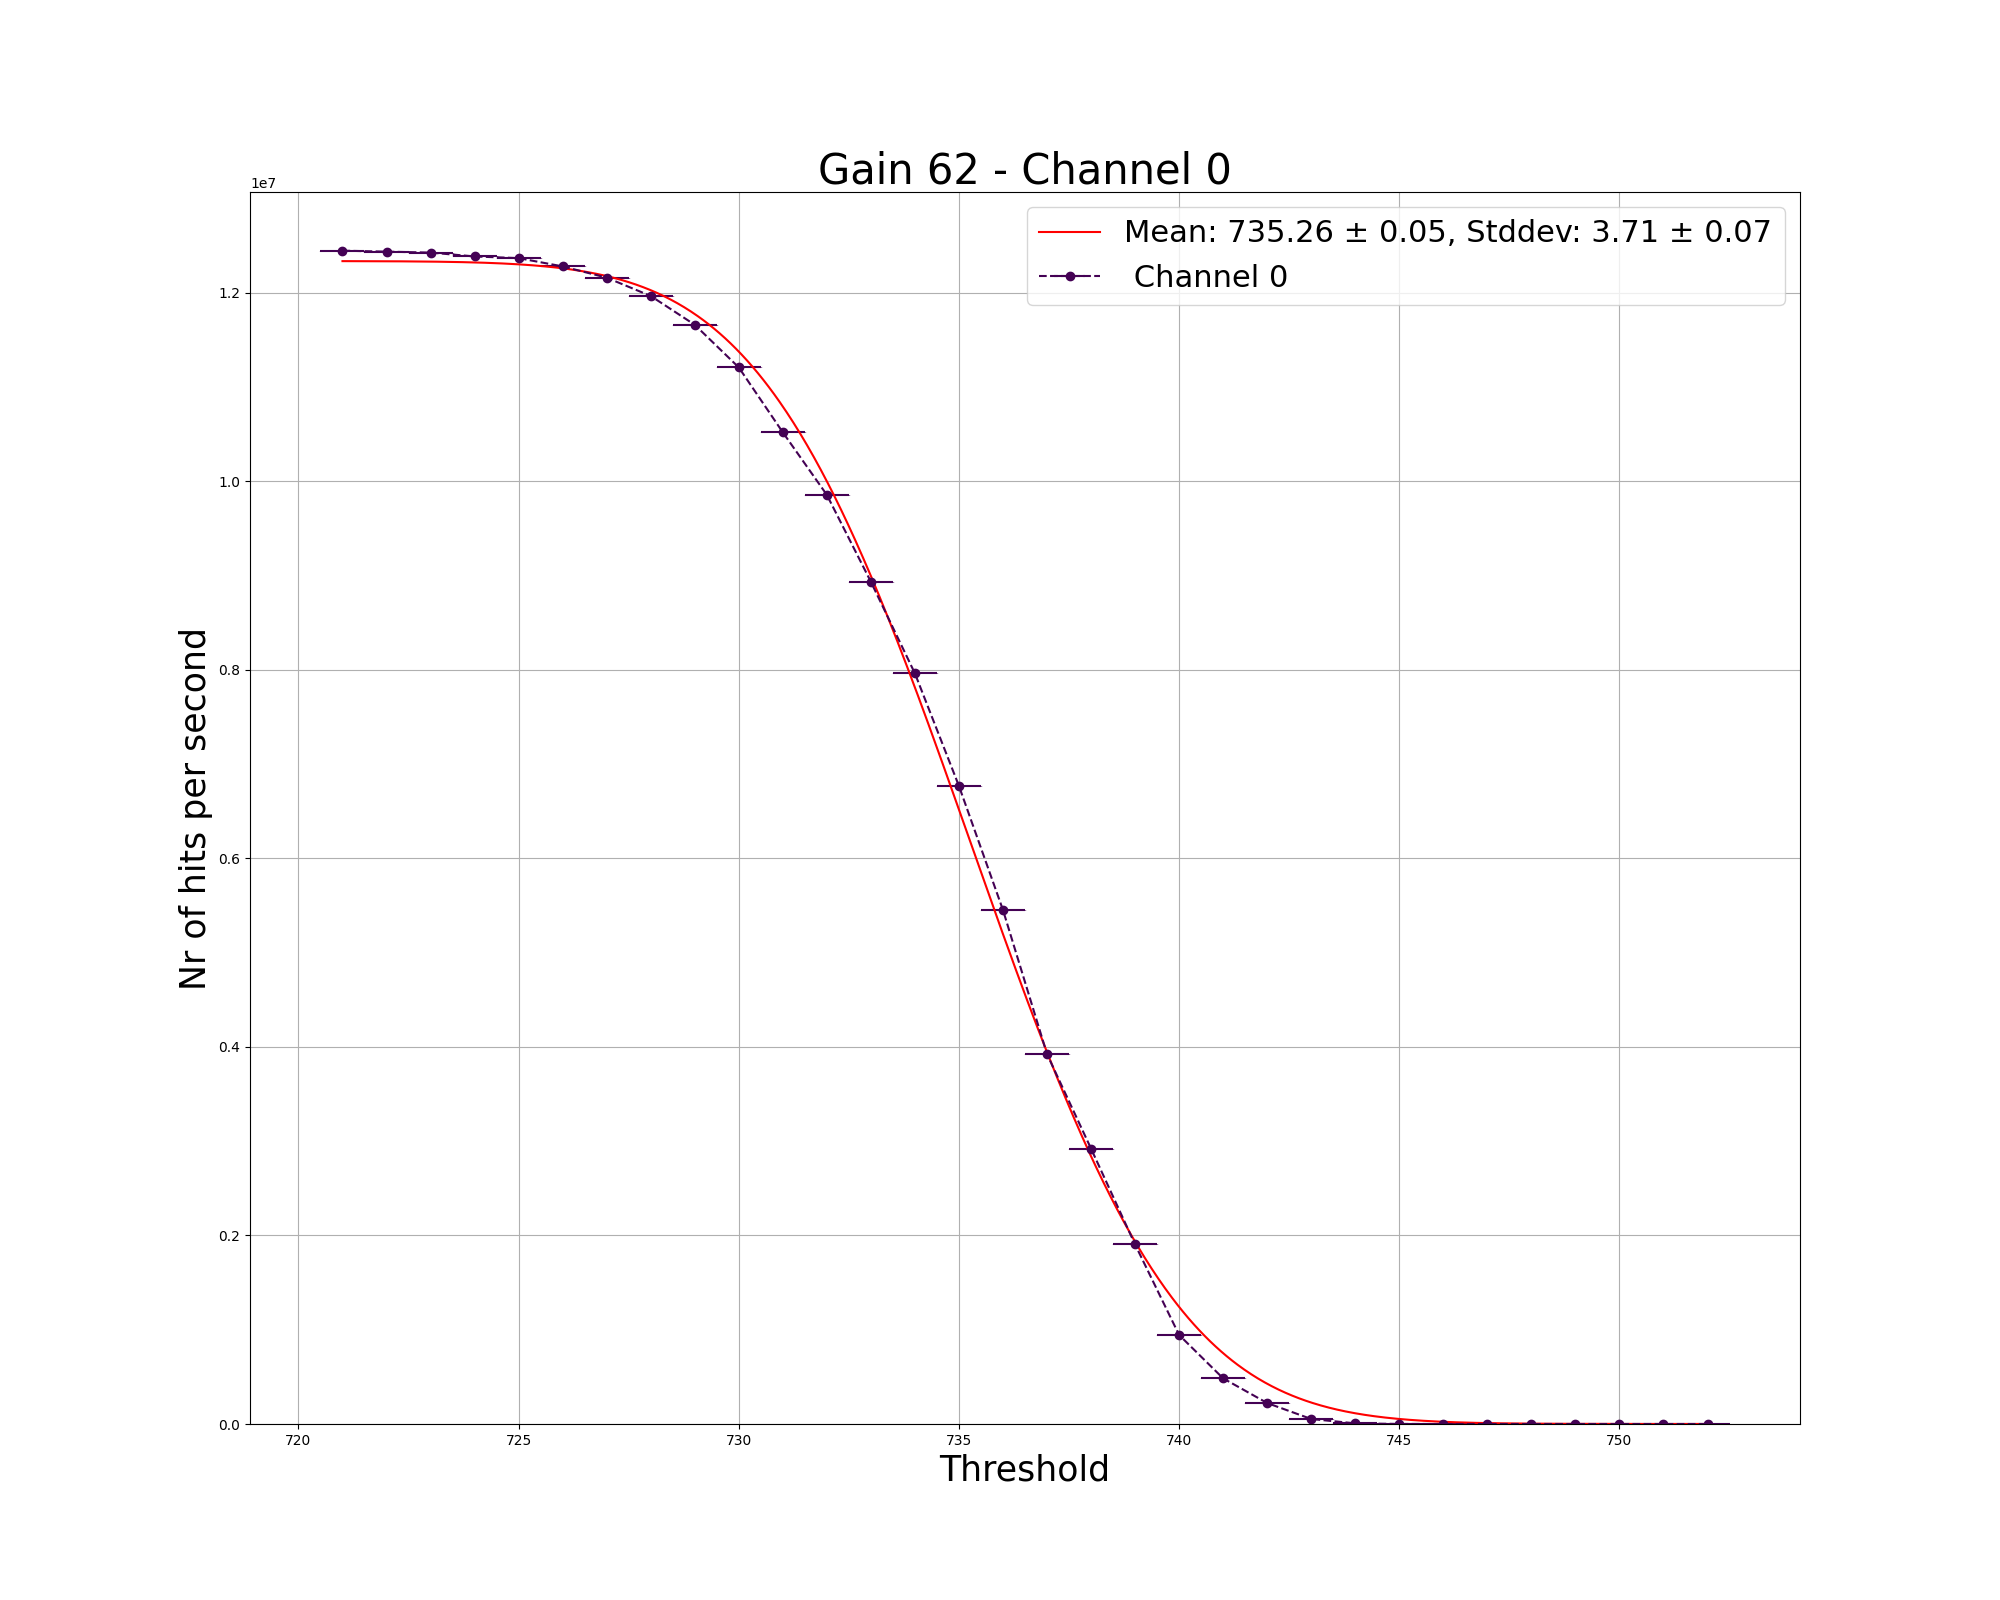
\includegraphics[width=0.6\textwidth]{Runs_170_400_Gain_62.0_0_ChannelALL_FPGAS.png}
    \caption{Results of the S-curve analysis for channel 0 of Citiroc1A 1 of FPGA 1 with gain 62.}
    \label{fig:S_curve_62}
\end{figure}
The S-curve fit, for all channels, for the high gain of 62 needed for the PRM experiment is shown in Figure \ref{fig:S_curve_62_ALL}. 

\begin{figure}[H]
    \centering
    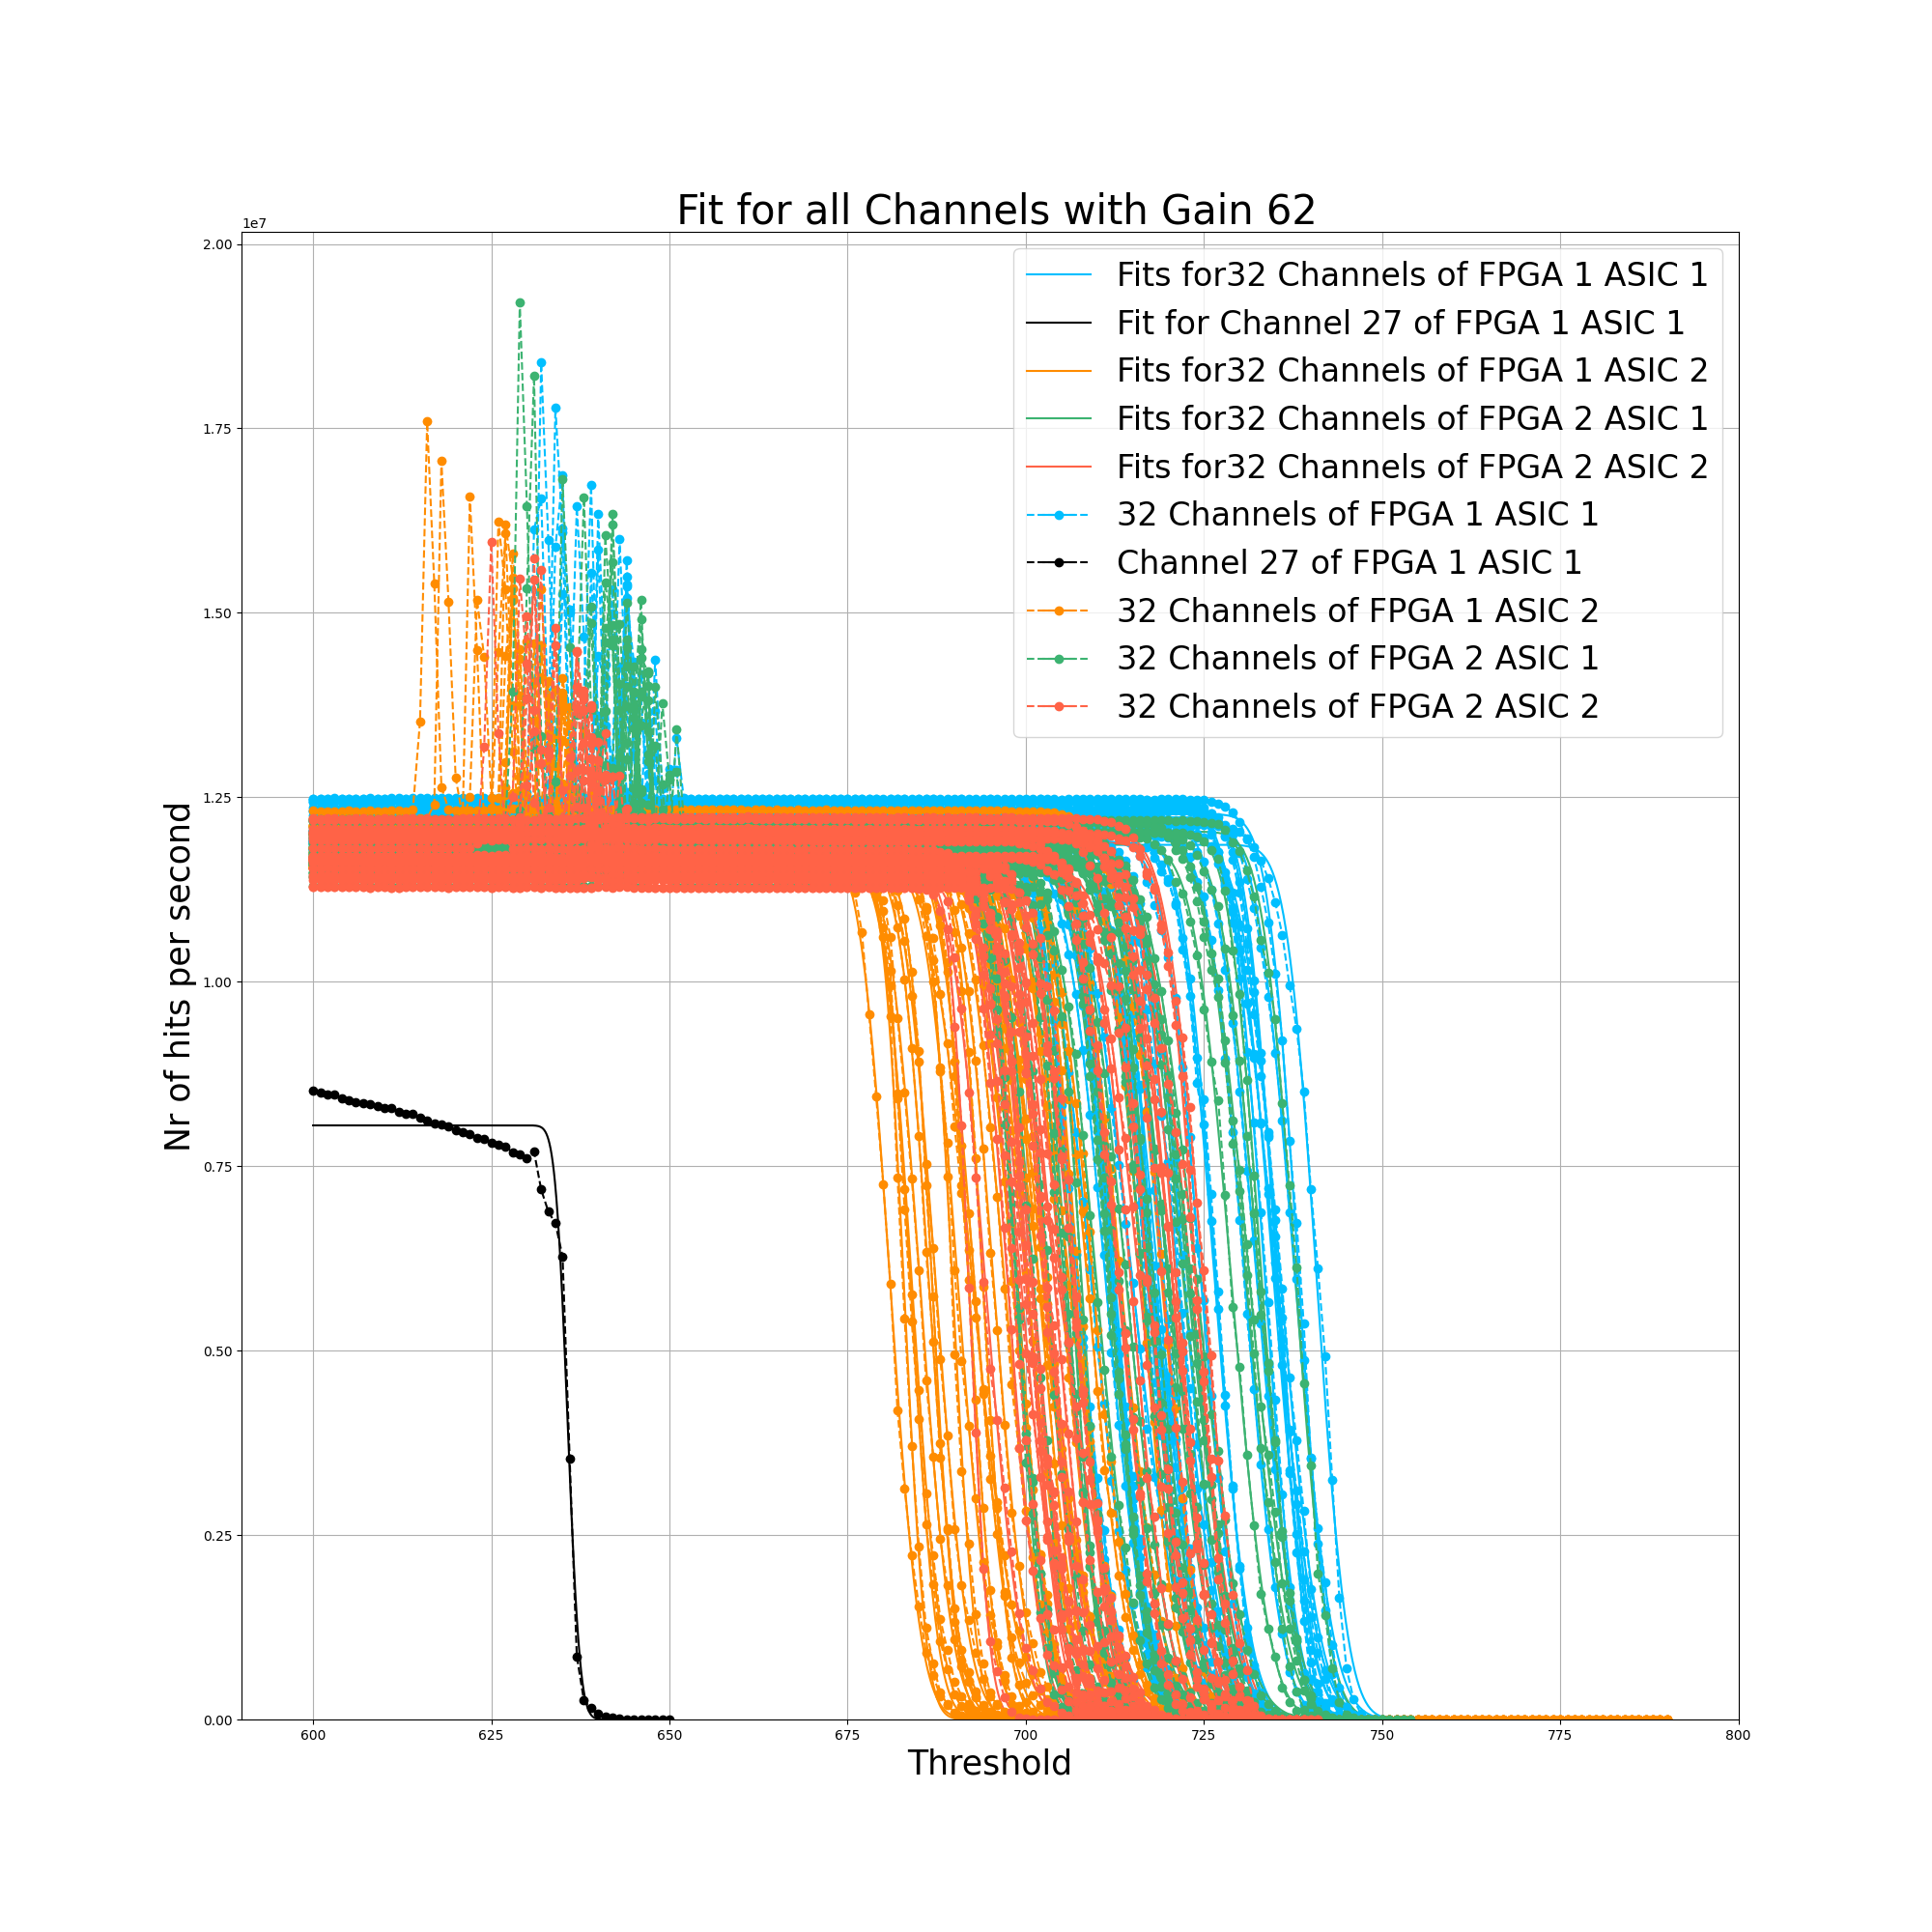
\includegraphics[width=0.69\textwidth]{Fit for all Channels with Gain 62 copy.png}
    \caption{Results of the S-curve analysis for all channels of the Citiroc1A ASICs of FPGA 1 and 2 with gain 62.}
    \label{fig:S_curve_62_ALL}
\end{figure}
The mean $\mu$ and the standard deviation $\sigma$ of the noise distribution that were determined from the S-curve fits and are shown in Appendix \ref{cha:appendixFitPar}.
They are plotted against the gain for all channels in Figure \ref{fig:Mean vs gain}.
\begin{figure}[H]
    \centering
    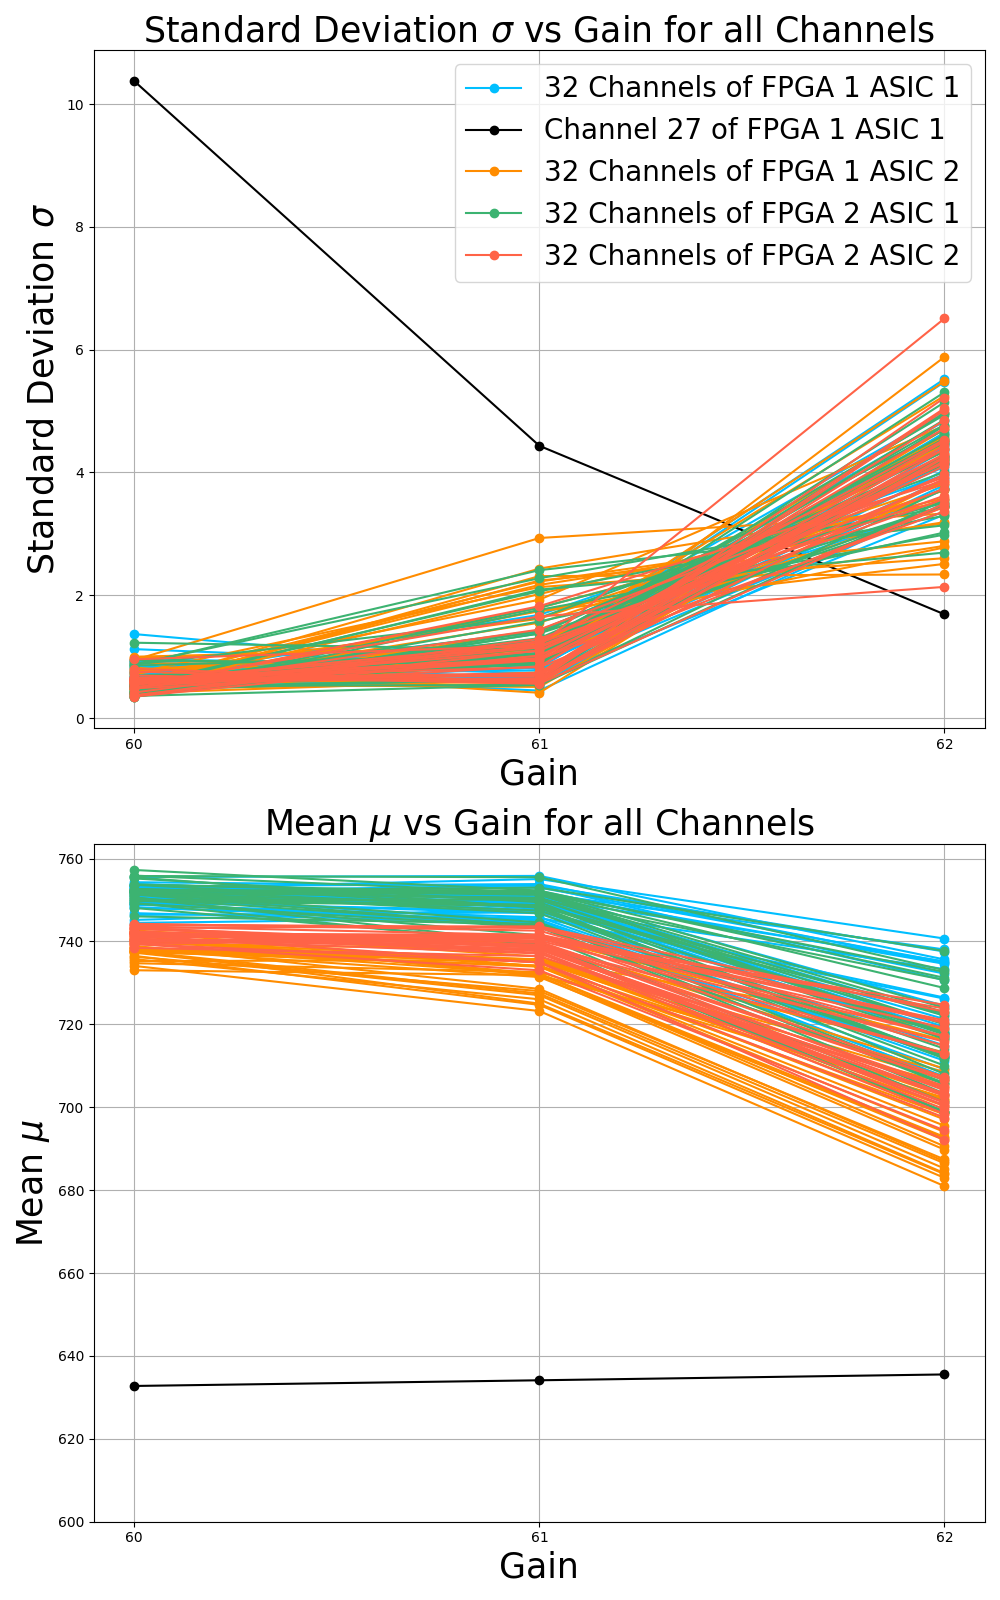
\includegraphics[width=0.6\textwidth]{Individual_Stddev_and_Mean_vs_Gain copy 2.png}
    \caption{Mean $\mu$ and standard deviation $\sigma$ determined from the S-curve fits for all channels of the Citiroc1A ASICs of FPGA 1 and 2 plotted vs the gain.}
    \label{fig:Mean vs gain}
\end{figure}

\subsection{Behavior at different Gain Setting}
The threshold scan of the Citiroc1A ASICs in the frontend electronics shows different behavior for gain ranges of 0 to 58 (Figure \ref{fig:threshold_scan_58}) and 60 to 62 (Figures \ref{fig:threshold_scan_60}, \ref{fig:threshold_scan_61} and \ref{fig:threshold_scan_62}),
with the threshold scan at gain 59 showing a transition between the two behaviors depicted in Figure \ref{fig:threshold_scan_59}.
This difference is also currently not understood and is suspected to have the same cause as the difference in the threshold scan compared to the testboard measurments. 
\newline
%This difference in behaviour is also observed in the S-curve analysis, with the mean $\mu$ and the standard deviation $\sigma$ of the noise distribution showing a jump between the two gain ranges and
%the the channels showing different behaviour at the transition point of gain 59. 
%This difference is visualized in Figure \ref{fig:Mean vs gain}.
A general trend of the standard deviation $\sigma$ of the S-curve increasing and the mean $\mu$ decreasing with higher gain is observed.
\subsection{Channel Behavior Analysis}
From the S-curve analysis it can be observed that the channels of the Citiroc1A ASICs show different behavior in the threshold scan.
\newline
Especially channel 27 of Citiroc1A 1 of FPGA 1 shows a significantly different behavior compared to the other channels,
as can be seen in Figure \ref{fig:Mean vs gain} and in the results of the threshold scan shown in the Figures \ref{fig:threshold_scan_60}, \ref{fig:threshold_scan_61} and \ref{fig:threshold_scan_62}.
\newline
Furthermore, for the threshold scan with gain 59 depicted in Figure \ref{fig:threshold_scan_59} , all the channels show diverging behavior, this is also suspected to be beacause of the transition between the two gain regions.
\newline
The behavior of channel 27 of Citiroc1A 1 of FPGA 1 seems to have a different cause than the gain transition and needs further investigation.
This could be investigated by performing a threshold scan with another FEE PCB and comparing the results.
\subsection{Summary of the Characterisation}
The threshold scan and the S-curve analysis show that the frontend electronics of the SFH are not performing as desired.
Due to this, a calibration of the individual channels of the frontend electronics is not yet possible.
The cause of the observed behavior is currently not understood and further investigation is required,
but a possible cause could be high frequency noise on the input signals of the Citiroc1A ASICs causing some unknown behavior of the ASIC.
Furthermore, the behavior of channel 27 of Citiroc1A 1 of FPGA 1 seems to have a different cause than the gain transition and also needs further investigation.

